\let\negmedspace\undefined
\let\negthickspace\undefined
\documentclass[journal,12pt,twocolumn]{IEEEtran}
\usepackage{cite}
\usepackage{amsmath,amssymb,amsfonts,amsthm}
\usepackage{algorithmic}
\usepackage{graphicx}
\usepackage{textcomp}
\usepackage{xcolor}
\usepackage{txfonts}
\usepackage{listings}
\usepackage{enumitem}
\usepackage{mathtools}
\usepackage{gensymb}
\usepackage{comment}
\usepackage[breaklinks=true]{hyperref}
\usepackage{tkz-euclide}
\usepackage{listings}
\usepackage{gvv}
\def\inputGnumericTable{}
\usepackage[latin1]{inputenc}
\usepackage{color}
\usepackage{array}
\usepackage{longtable}
\usepackage{calc}
\usepackage{multirow}
\usepackage{hhline}
\usepackage{ifthen}
\usepackage{lscape}

\newtheorem{theorem}{Theorem}[section]
\newtheorem{problem}{Problem}
\newtheorem{proposition}{Proposition}[section]
\newtheorem{lemma}{Lemma}[section]
\newtheorem{corollary}[theorem]{Corollary}
\newtheorem{example}{Example}[section]
\newtheorem{definition}[problem]{Definition}
\newcommand{\BEQA}{\begin{eqnarray}}
\newcommand{\EEQA}{\end{eqnarray}}
\newcommand{\define}{\stackrel{\triangle}{=}}
\theoremstyle{remark}
\newtheorem{rem}{Remark}
\begin{document}

\bibliographystyle{IEEEtran}
\vspace{3cm}

\title{NCERT Discrete - 11.5.9.2}
\author{EE23BTECH11201 - Abburi Tanusha$^{*}$% <-this % stops a space
}
\maketitle
\newpage
\bigskip

\renewcommand{\thefigure}{\theenumi}
\renewcommand{\thetable}{\theenumi}

\vspace{3cm}

\maketitle
\textbf{Question:} 
The sum of three numbers in an arithmetic progression (AP) is $24$ and the product of those three numbers is $440$, find the values of the three numbers.

\solution
The following information is provided in the question:
\begin{table}[h]
 	\centering
 	\resizebox{6 cm}{!}{
 		

    \begin{tabular}{|c|c|c|}
        \hline
        \textbf{Parameter} & \textbf{Value} & \textbf{Description} \\
        \hline
        a     & 8 & First term \\
        d     & 5 & common difference\\
        xi(0) & 8 & First term \\
        \hline
    \end{tabular}
    
    



 	}
 	\vspace{6 pt}
 	\caption{Parameters}
 	\label{tab:my_label} 
 \end{table}
\newline
Let the three numbers in the arithmetic progression be denoted as $x(0)$, $x(1)$, and $x(2)$.
\newline
From Table \ref{tab:my_label}
\begin{align}
  x(0) + x(1) + x(2) &= 24 \\
   \brak{x(1) - d} + x(1) + \brak{x(1) + d} &= 24 \\
    3x(1) &= 24 \\ 
   \implies x(1) &= 8 
\end{align}
\begin{align}
   x(0) \cdot x(1) \cdot x(2) &= 440  \\
 \brak{8-d} \cdot \brak{8} \cdot \brak{8+d} &= 440  \\
 \brak{8-d} \cdot \brak{8+d} &= 55 \\
 64-d^2 &= 55 \\
  \implies d &= 3 \\
  \implies x(0) &= 5
\end{align}
\begin{align}
     x(n) &= \brak{5 + 3n}u(n)  
 \end{align}
 From equation \eqref{eq:11.9.5.26.2}:  
\begin{align}      
  X(z) = \frac{5 - 8z^{-1}}{(1-z^{-1})^2} ; \quad \abs{z} > \abs{1}  
\end{align}
Therefore, the required three numbers in AP are $5$, $8$, and $11$.
\begin{figure}[h!]
  \centering
  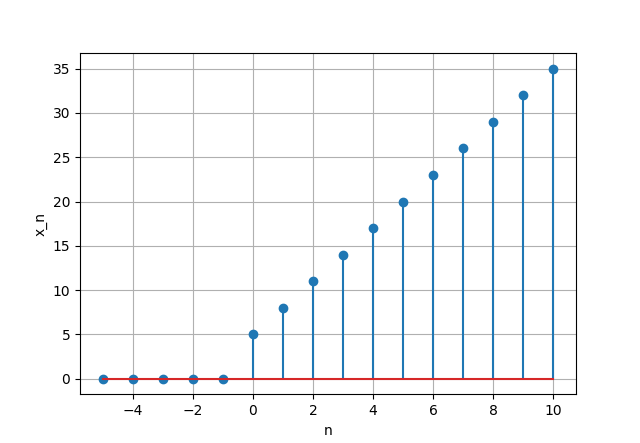
\includegraphics[width=\columnwidth]{figs/stem_plot.png} 
  \label{fig:1}
  \caption{stem plots of x(n)}
\end{figure}
\end{document}

